\subsection{Ecore Editors}\label{sec:ecore-editors}

This section describes some of the existing editors for \gls{Ecore} models.
Most of them are provided in the \gls{Eclipse}.
They can be used to draw inspiration for new \gls{cloud} editors, and suggest functionalities and requirements that are needed.

\subsubsection{Sample Reflective Ecore Model Editor} %Default EMF Genmodel editor
A master-detail tree editor in \gls{Eclipse}.
It uses the \emph{reflective \acrshort{API}} of \gls{Ecore} to convert models into trees.
It is \gls{open source}\footnote{Sample Reflective editor source: \href{https://git.eclipse.org/c/emf/org.eclipse.emf.git/tree/plugins/org.eclipse.emf.ecore.editor}{https://git.eclipse.org/c/emf/org.eclipse.emf.git/tree/plugins/org.eclipse.emf.ecore.editor}.}
The source code lives in the \href{https://git.eclipse.org/c/emf/org.eclipse.emf.git/tree/plugins/org.eclipse.emf.ecore.editor/src/org/eclipse/emf/ecore/presentation/EcoreEditor.java}{org.eclipse.emf.ecore.editor} package, (indicating that it was generated by a \texttt{genmodel}\footnote{Some source code also has \texttt{@generated} annotations, confirming this.}).

A screenshot of the editor can be seen in \cref{fig:sample-reflective-ecore-model}.
It supports both models (\cref{sfig:sample-reflective-ecore-model-screenshot}) and model instances (\cref{sfig:sample-reflective-ecore-model-instance-screenshot}).

A relevant piece of the source code is the \texttt{ReflectiveItemProvider}\footnote{\href{https://git.eclipse.org/c/emf/org.eclipse.emf.git/tree/plugins/org.eclipse.emf.edit/src/org/eclipse/emf/edit/provider/ReflectiveItemProvider.java}{https://git.eclipse.org/c/emf/org.eclipse.emf.git/tree/plugins/org.eclipse.emf.edit/src/org/eclipse/emf/edit/provider/ReflectiveItemProvider.java}} from \texttt{org.eclipse.emf.edit}.
This code converts the model instances to text labels (\href{https://git.eclipse.org/c/emf/org.eclipse.emf.git/tree/plugins/org.eclipse.emf.edit/src/org/eclipse/emf/edit/provider/ReflectiveItemProvider.java#n390}{line 390}) and provides their icons (\href{https://git.eclipse.org/c/emf/org.eclipse.emf.git/tree/plugins/org.eclipse.emf.edit/src/org/eclipse/emf/edit/provider/ReflectiveItemProvider.java#n380}{line 380}), for display in a tree.
% https://git.eclipse.org/c/emf/org.eclipse.emf.git/tree/plugins/org.eclipse.emf.edit/model/Tree.ecore

\begin{figure}
    \centering
    \begin{subfigure}[b]{.45\textwidth}
        \centering
        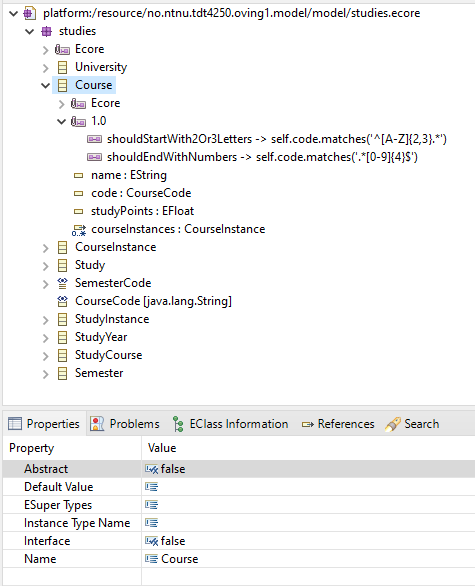
\includegraphics[width=\textwidth]{figures/ecore-sample-reflective-ecore-model-editor}
        \caption{A model opened in the editor.}
        \label{sfig:sample-reflective-ecore-model-screenshot}
    \end{subfigure}
    \hfill
    \begin{subfigure}[b]{.45\textwidth}
        \centering
        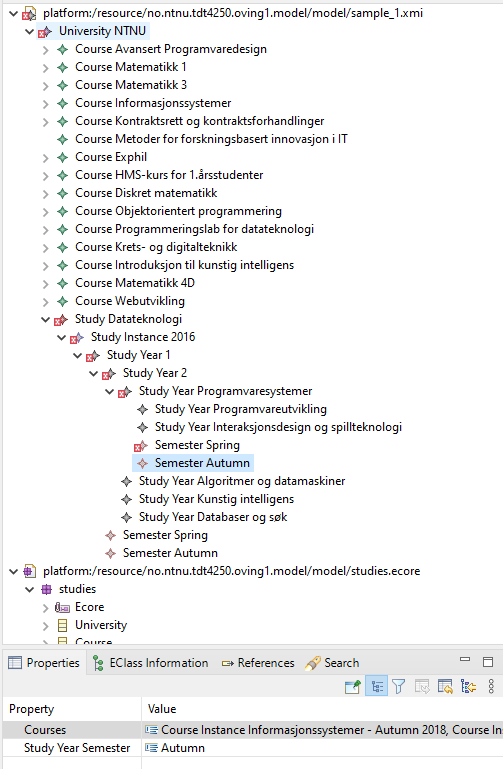
\includegraphics[width=\textwidth]{figures/ecore-sample-reflective-ecore-model-editor-instance.png}
        \caption{A \emph{dynamic instance} (\gls{XMI}) opened in the editor.}
        \label{sfig:sample-reflective-ecore-model-instance-screenshot}
    \end{subfigure}
    \caption{Screenshots of the Sample Reflective Ecore Model Editor in \gls{Eclipse}.}\label{fig:sample-reflective-ecore-model}
\end{figure}


\subsubsection{EMF Forms Ecore Editor} % EMF Forms based
The \emph{EMF Forms Ecore Editor} is based on \emph{EMF Forms}\footnote{\href{https://eclipsesource.com/blogs/tutorials/emf-forms-editors/}{https://eclipsesource.com/blogs/tutorials/emf-forms-editors/}}, a library to create form editors for \gls{Ecore} models.
It runs in \gls{Eclipse} and is \gls{open source}\footnote{EMF Forms source: \href{https://git.eclipse.org/c/emfclient/org.eclipse.emf.ecp.core.git/tree/bundles/org.eclipse.emfforms.editor.ecore}{https://git.eclipse.org/c/emfclient/org.eclipse.emf.ecp.core.git/tree/bundles/org.eclipse.emfforms.editor.ecore}.}.
The editor supports both \texttt{.ecore}, \texttt{.xmi} and \texttt{.genmodel} files.
It has a generic editor for all \gls{XMI} files\footnote{\emph{Generic XMI Editor} in \gls{Eclipse}.}, and specialized editors for ecore\footnote{\emph{Ecore Editor} in \gls{Eclipse}.} and genmodel.~\cite{eclipsesourceEMFFormsEditors2016}

A screenshot can be seen in \cref{fig:emf-forms-ecore-editor}.

\begin{figure}[htbp]  % order of priority: h here, t top, b bottom, p page
  \centering
  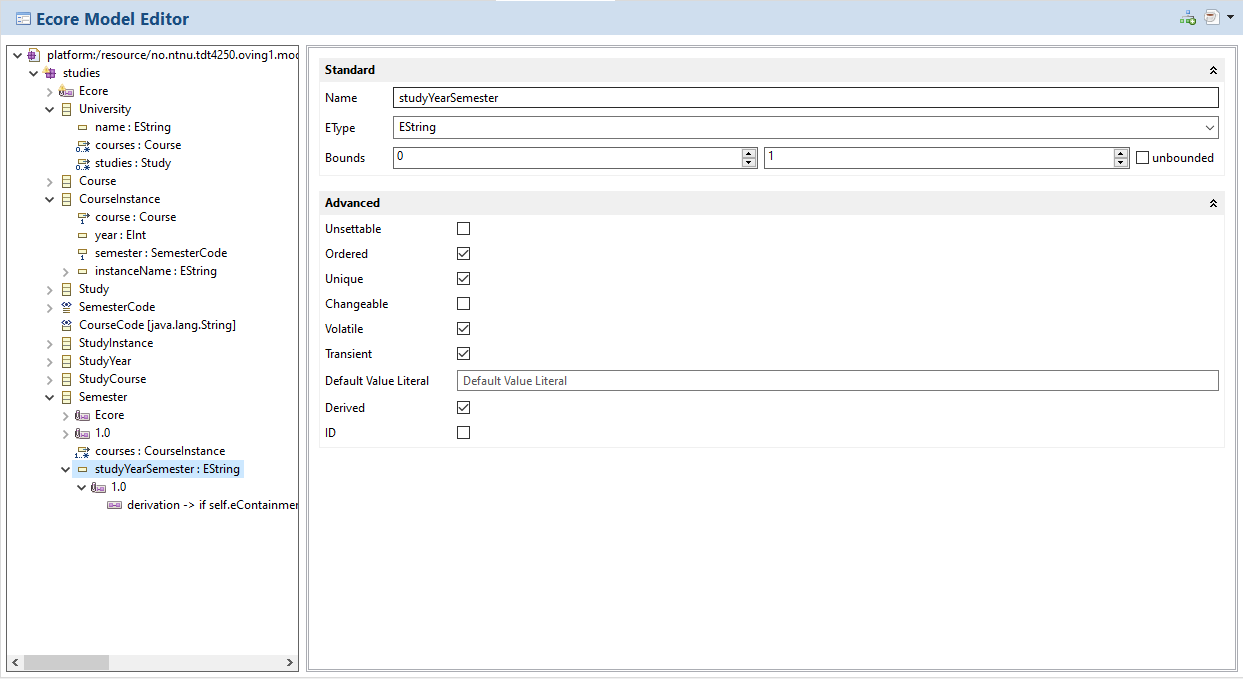
\includegraphics[width=\textwidth]{figures/ecore-eclipse-emf-forms-model-editor.png}
  \caption[EMF Forms Ecore Editor]{A screenshot of a model in the EMF Forms based Ecore Editor.}\label{fig:emf-forms-ecore-editor}
\end{figure}



\subsubsection{Ecore Tools} % Sirius based
The \emph{Ecore Tools} editor is based on Sirius (see \cref{sec:sirius}).
It displays diagrams as \gls{UML} Class Diagrams in the \gls{Eclipse}.
The editor is \gls{open source}\footnote{Ecore Tools source: \href{https://git.eclipse.org/r/plugins/gitiles/ecoretools/org.eclipse.ecoretools/}{https://git.eclipse.org/r/plugins/gitiles/ecoretools/org.eclipse.ecoretools/}.}

A screenshot of the Ecore Tools editor is shown in \cref{fig:ecore-tools-screenshot}.

\begin{figure}[htbp]  % order of priority: h here, t top, b bottom, p page
  \centering
  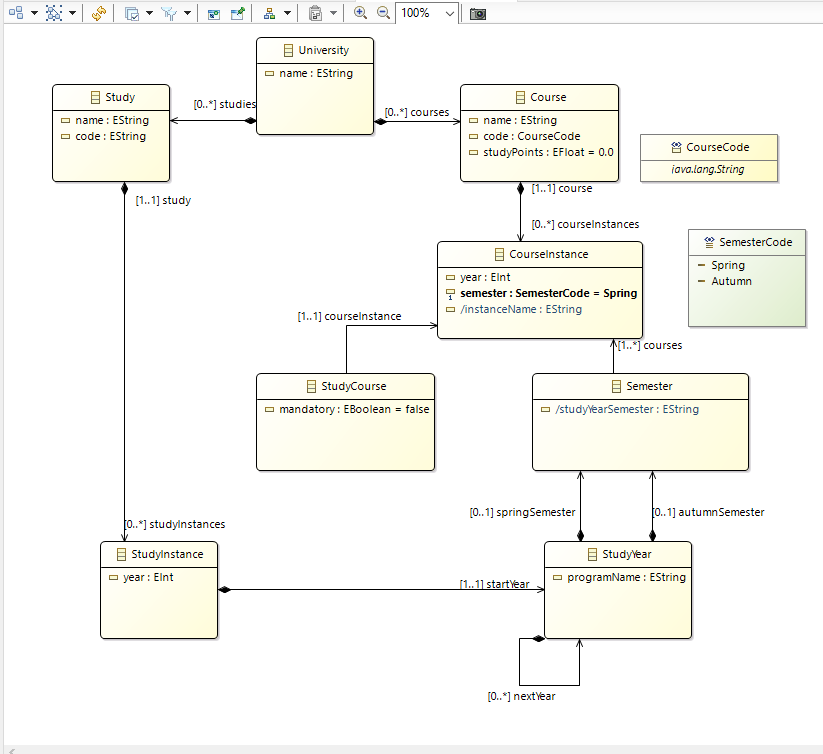
\includegraphics[width=\textwidth]{figures/ecore-eclipse-sirius-aird-graphical-editor.png}
  \caption[Ecore Tools Screenshot]{Ecore Tools in \gls{Eclipse} with a model opened.}\label{fig:ecore-tools-screenshot}
\end{figure}


\subsubsection{EMF.Cloud --- ecore-glsp}\label{sec:ecore-glsp} %Theia
The \emph{ecore-glsp} is an \gls{open source}\footnote{ecore-glsp source: \href{https://github.com/eclipse-emfcloud/ecore-glsp}{https://github.com/eclipse-emfcloud/ecore-glsp}.} \gls{Theia} \emph{Extension} (\cref{sec:theia-extension}) originally created by EclipseSource.
The project was donated to Eclipse EMF.Cloud.
It renders \gls{Ecore} models as diagrams, similar to Ecore Tools.

The extension is made using \gls{GLSP} (\cref{sec:glsp}) and Sprotty (\cref{sec:sprotty}).
When using the plugin, diagram layouts are persisted to a separate \texttt{.enotation} \gls{XMI} file.~\cite{camilleletavernierEclipseemfcloudEcoreglsp2020}

Although it only supports \gls{Theia} now, a developer using the \gls{GLSP} integration for \gls{VSCode} could possibly adapt it to a VSCode extension (see \cref{sec:vscode-extension}). A \gls{VSCode} integration library is created by EclipseSource\footnote{VSCode glsp integration source: \href{https://github.com/eclipsesource/glsp-vscode-integration}{https://github.com/eclipsesource/glsp-vscode-integration}.}.

The scope of the ecore-glsp library seems to extend beyond just diagrams.
The Github issues\footnote{Tree editor issue: \href{https://github.com/eclipse-emfcloud/ecore-glsp/issues/45}{https://github.com/eclipse-emfcloud/ecore-glsp/issues/45}.}\footnote{Model server issue: \href{https://github.com/eclipse-emfcloud/ecore-glsp/issues/28}{https://github.com/eclipse-emfcloud/ecore-glsp/issues/28}.}\footnote{Property view issue: \href{https://github.com/eclipse-emfcloud/ecore-glsp/issues/53}{https://github.com/eclipse-emfcloud/ecore-glsp/issues/53}.} indicate that the developers want to add a tree editor, property view, validation and a model server.
The issue for a tree editor suggest using the \emph{Theia Tree Editor} component (see \cref{sec:theia-tree-editor}).
However, if they add the Theia Tree Editor, the library \textit{may} lose compatibility with other \glspl{IDE} than \gls{Theia}, such as \gls{VSCode}.
Alternatively, the features will only be available in the \gls{Theia} client.

% CrossEcore Ecore editor
% https://github.com/crossecore/ecore-editor
% TODO: Write
% Typescript, ELKjs, Sprotty, Monaco and React